\chapter{Referencial Teórico} \label{cap:referencial-teorico}
Este Capítulo apresenta a fundamentação teórica relativa a este trabalho. Para tanto, o Capítulo encontra-se organizado da seguinte maneira: na Seção \ref{sec:spark} é explicado o \textit{framework} Apache Spark juntamente com o modelo de memória utilizado. A Seção \ref{sec:Zookeeper} é dedicada à apresentação do Apache ZooKeeper. Por fim, a Seção \ref{sec:trab-relacionados} tem como objetivo explanar trabalhos relacionados a este, encontrados na literatura.

\section{Apache Spark}\label{sec:spark}
O Spark é um \textit{framework} de código aberto, projetado com o objetivo de realizar o processamento de dados massivos de maneira paralela e distribuída. A criação de aplicações Spark é realizada através de uma API (\textit{Application Program Interface}) disponibilidada pelo \textit{framework}. 

Através desta API, é possível criar e manipular RDDs \cite{karau2015learning}, utilizando transformações e ações. As transformações são métodos que recebem um RDD como entrada e geram um ou mais RDDs como saída. São exemplos de transformações os métodos \textit{map} e \textit{filter}. Enquanto o método \textit{map} aplica uma mesma função para todos os dados do \textit{dataset} contido no RDD, o método \textit{filter} realiza um filtro neste conjunto de dados, obedecendo uma condição definida pelo desenvolvedor. 

As ações são operações cujo objetivo é computar o RDD e gerar um valor, como é caso dos métodos \textit{reduce} e \textit{count}. O método \textit{reduce} agrega o conjunto de dados do RDDs em um único valor. Já o método \textit{count} realiza uma contagem do número de registros armazenados no RDD.

Juntamente com os métodos de transformações e ações, são disponibilizados ao desenvolvedor métodos auxiliares a fim de realizar o armazenamento de RDDs, permitindo que estes sejam mantidos em \textit{cache} após sua computação. A possibilidade de realizar a persistência dos dados evita que o RDD seja recomputado a cada reutilização em computações futuras. Neste sentido, dois métodos podem ser utilizados: \textit{cache()} e \textit{persist()}. O método \textit{cache()} armazena os dados em memória principal, sendo este o nível padrão para armazenamento dos dados em \textit{cache}. Por outro lado, o método \textit{persist()} permite que seja especificado o nível de armazenamento, isto é, memória, disco ou combinação de ambos, para manter as partições em \textit{cache}.

Internamente, um RDD é composto por:
\begin{itemize}
    \item[a)] uma lista de partições responsáveis por armazenar os dados. Geralmente, uma partição do RDD corresponde a um bloco de dado armazenado no HDFS (\textit{Hadoop Distributed File System)}, com tamanho padrão de até 128 MB para o Hadoop (versão 2);
    \item[b)] uma função para computar cada partição;
    \item[b)] uma lista de dependência de outros RDDs;
    \item[b)] opcionalmente, um particionador para RDDs chave-valor (isto é, hash-particionado) e;
    \item[b)] uma lista de locais preferidos no \textit{Cluster} para realizar a computação de cada partição, sendo este atributo opcional.
\end{itemize}

A avaliação dos RDDs criados é realizada de forma \textit{lazy}, ou seja, sua computação não é efetuada no momento de sua criação, sendo processados apenas quando for necessário. Quando um novo RDD é gerado, este carrega consigo uma referência do(s) RDD(s) ancestral(is), adicionado(s) a sua lista de dependências. Tal processo é realizado na criação de qualquer RDD, gerando o grafo direcionado acíclico de dependências da aplicação.

O grafo direcionado acíclico (DAG -- \textit{Directed Acyclic Graph}), denominado de \textit{lineage} do RDD, é utilizado para realizar a computação do RDD juntamente com suas respectivas dependências. Este grafo constitui um importante mecanismo de recuperação de falhas implementado pelo Spark. Assim, em situações onde partições são perdidas, o sistema pode realizar a recomputação dos dados a partir de uma réplica restante dos dados de entrada \cite{karau2015learning}.

Ao ser aplicada uma ação a um determinado RDD, este é submetido ao escalonador do Spark, denominado \textit{DAGScheduler}, com o objetivo de transformar a sua \textit{lineage} em um plano de execução físico composto por estágios. Para a criação destes estágios, o \textit{DAGScheduler} particiona o grafo do RDD em limites \textit{shuffle}, isto é, em limites onde há redistribuição dos dados entre partições. 

Dependências onde não há redistribuição de dados são enfileiradas em um mesmo estágio para serem computadas, como é o caso das transformações \textit{map} e \textit{filter}. Em contrapartida, dependências \textit{shuffle} requerem dois estágios para serem computadas, sendo o primeiro estágio para realizar a escrita dos arquivos de saída e um segundo estágio para ler estes dados, após uma barreira de sincronização entre as operações, \cite{DAGSchedulerSpark}. 

O procedimento de criação do plano de execução da aplicação, denominado de \textit{job}, é realizado sempre que uma ação é aplicada a um determinado RDD. Assim, a execução de uma mesma aplicação pode ser dividida em diversos \textit{jobs} até a sua completa finalização.

Após ser gerado o plano de execução físico pelo \textit{DAGScheduler}, o Spark executa os estágios da aplicação distribuindo o processamento. Esta execução é feita através de \textit{tasks}. Uma \textit{task} consiste na menor unidade de computação possível, onde cada uma destas representa uma computação responsável por executar a mesma fatia de código, mas em diferentes porções dos dados da aplicação. \cite{karau2017high}.

\subsection{Arquitetura do \textit{Framework}}
Para realizar o processamento de aplicações, o Spark  utiliza o modelo \textit{Master} e \textit{Worker} (Mestre e Trabalhador) para seu funcionamento do \textit{cluster}. Deste modo, sua arquitetura é composta basicamente por três componentes: \textit{Driver Program}, \textit{Cluster Manager} e \textit{Worker}, conforme ilustra a Figura \ref{fig:spark_arquitetura}.

O \textit{Driver Program} é responsável por hospedar o contexto da aplicação em um processo na \textit{Java Virtual Machine} (JVM), sendo contido no nodo \textit{Master} do \textit{Cluster}. Além disso, o \textit{Driver} é responsável por armazenar o escalonador do Spark (DAGScheduler) e gerenciar os \textit{jobs} da aplicação Spark. 

\begin{figure}[!ht]
    \caption{Arquitetura do Apache Spark.}
    \begin{center}
        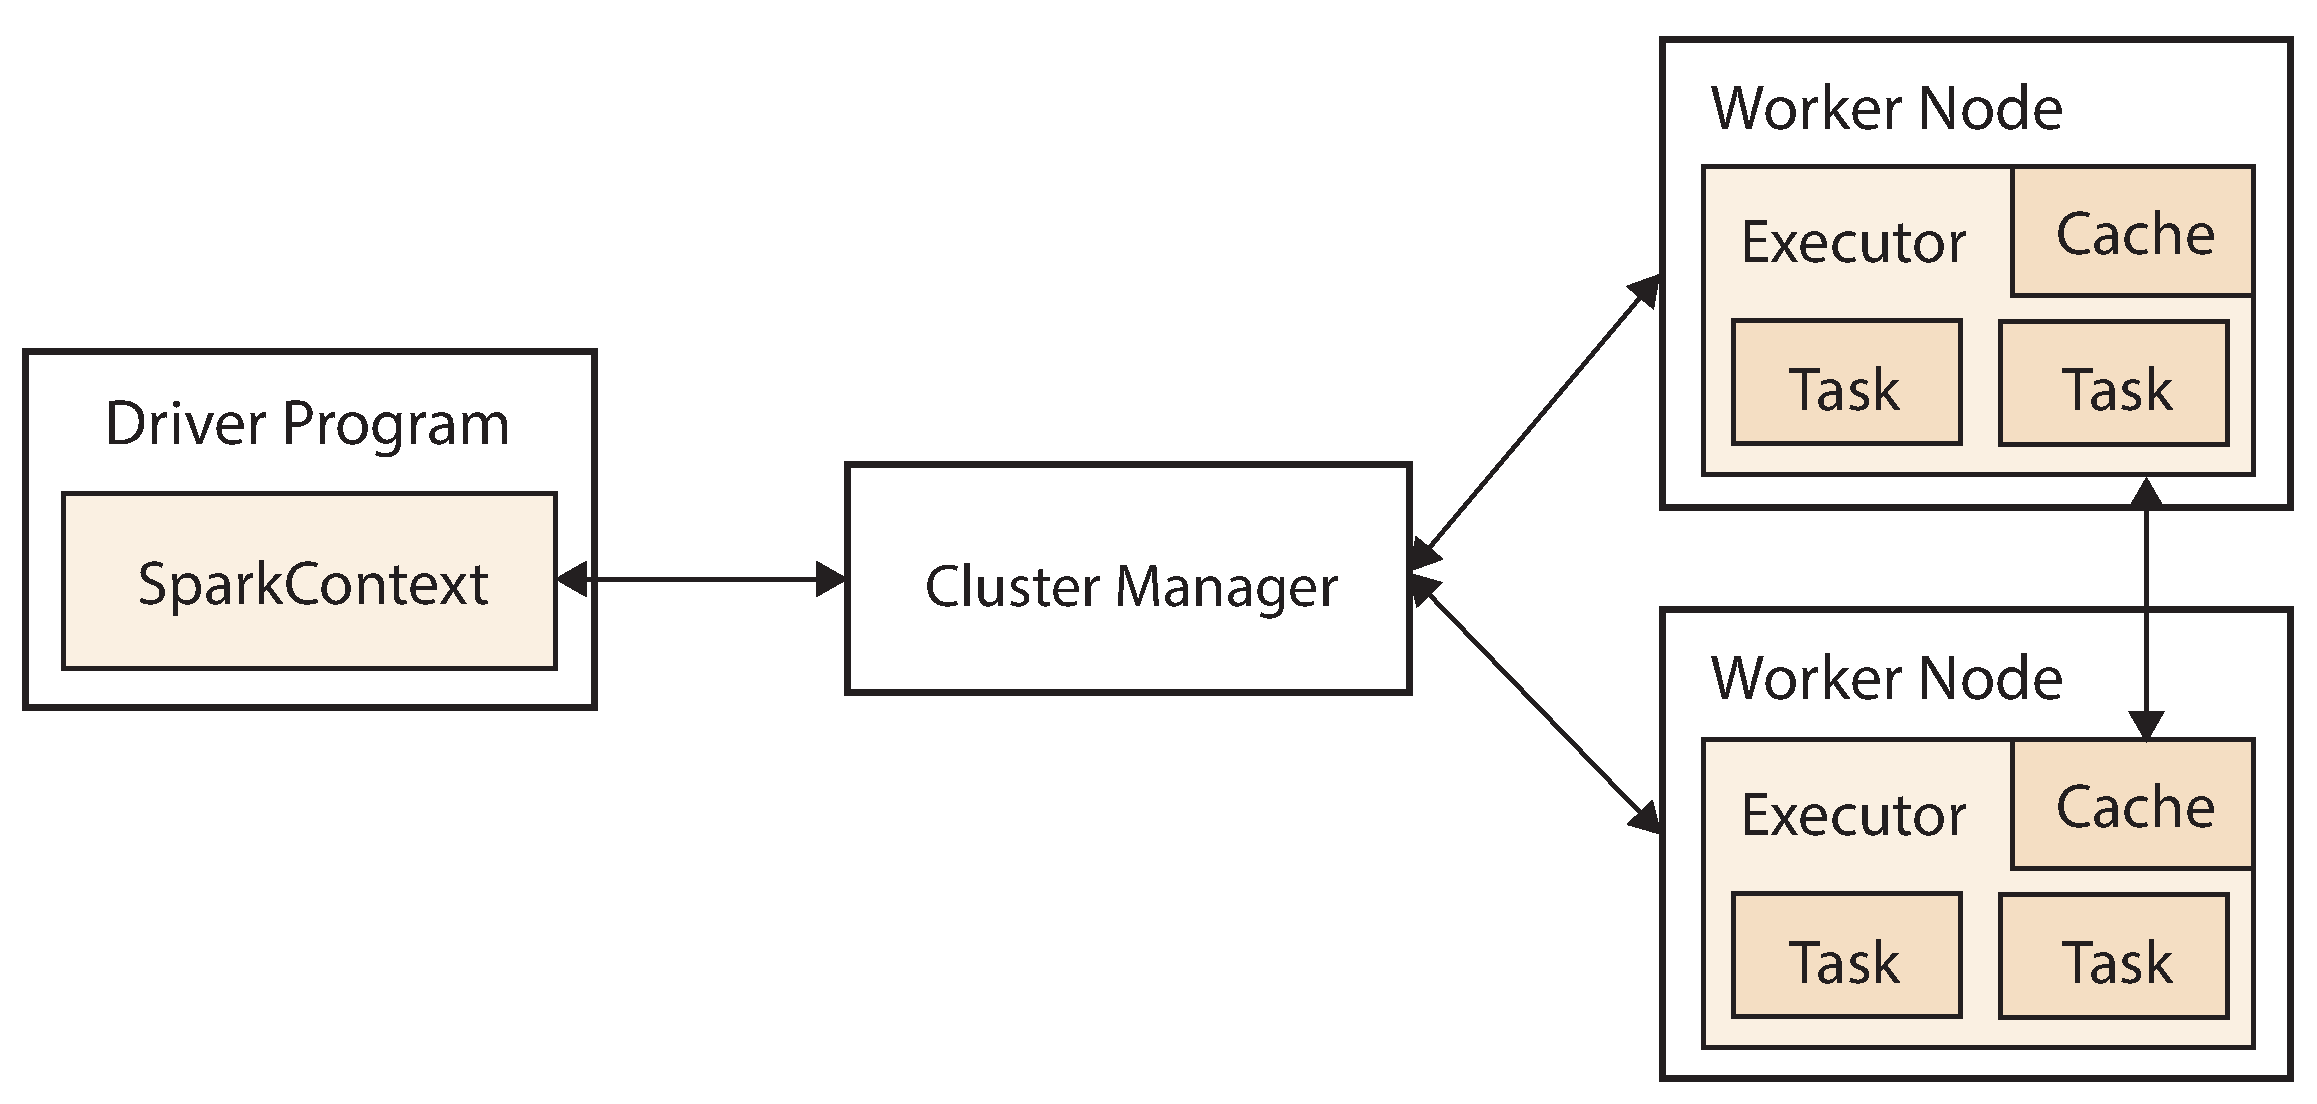
\includegraphics[scale=0.32]{imagens/spark_arquitetura.pdf}
    \end{center}
    \small{Fonte: Adaptado de (\citeauthor{frampton2015mastering}, 2015, p. 8)}
    \label{fig:spark_arquitetura}
\end{figure}


O \textit{Cluster Manager} é encarregado de gerenciar as máquinas que serão utilizadas como \textit{Workers} durante o processamento das aplicações Spark. De acordo \cite{chambers2018spark}, são esses gerenciadores de \textit{Clusters} que concedem recursos para completar a execução da aplicação. Por padrão, o Spark inclui um gerenciador de recursos \textit{stand-alone} incluso na distribuição  do \textit{framework}. Além deste, há suporte para o Apache Hadoop YARN\footnote{Disponível em: https://hadoop.apache.org}, Apache Mesos\footnote{Disponível em: http://mesos.apache.org/} e Kubernetes\footnote{Disponível em: https://kubernetes.io/}.

Os \textit{Workers} são os nodos que realizam o processamento das \textit{tasks} necessárias para a computação do \textit{job}, sendo estes nodos os encarregados de armazenar os \textit{Executors} do Spark. Um \textit{Executor} consiste em um processo JVM isolado lançado pelo Spark, com o objetivo executar o código delegado pelo \textit{Driver Program} e reportar seu \textit{status}. Além disso, cada \textit{Executor} possui sua região de memória isolada capaz de prover o armazenamento em memória para RDDs. O gerenciamento deste espaço é feito de forma autônoma pelo próprio \textit{Executor}, utilizando o algoritmo LRU.

\subsection{Modelo de Divisão da Memória}
O espaço de memória alocado e gerenciado por cada \textit{Executor} pode ser dividio em  três principais regiões de memória: Reservada, Usuário e Spark. Esta divisão pode ser observada na Figura \ref{fig:spark_memoria_arquitetura}.

\begin{figure}[!ht]
    \caption{Arquitetura da Memória do Apache Spark.}
    \begin{center}
        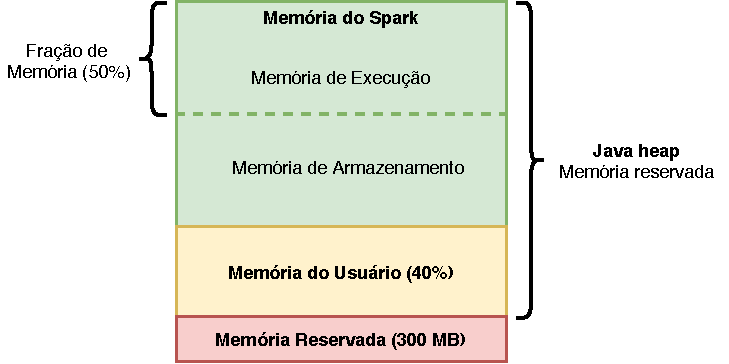
\includegraphics{imagens/modelo_memoria_spark_corrigido_2.pdf}
    \end{center}
    \small{Fonte: Adaptado de \cite{UnifiedMemoryManager}}
    \label{fig:spark_memoria_arquitetura}
\end{figure}

A Memória Reservada é uma região alocada estaticamente, via código fonte, com tamanho igual a 300MB, não sendo incluída no cálculo de memória disponível no Spark. O principal objetivo dessa área de memória é armazenar objetos internos do Spark.

A Memória do Usuário é a fração do \textit{Java heap} disponível para o usuário utilizar. Nessa região são armazenadas as estruturas, objetos e dados criados durante o desenvolvimento de aplicações Spark. O tamanho desta região corresponde a 40\% da memória disponível após a alocação da memória reservada. É importante ressaltar que o gerenciamento desta memória não é realizado pelo Spark, sendo delegado inteiramente ao \textit{Garbage Collector} (GC) da JVM.

A Memória do Spark é a região efetivamente controlada e gerenciada pelo Spark e GC da JVM. O tamanho desta região corresponde à fração de 60\% da memória disponível do \textit{Java heap} após a alocação da Memória Reservada. Esta região é subdividida em duas porções: Memória de Execução e Memória de Armazenamento, cada qual com 50\% do tamanho da área inicial da Memória do Spark. 

A Memória de Execução é responsável por armazenar os objetos e dados resultantes de operações intermediárias durante a execução de \textit{tasks}. Já a Memória de Armazenamento abriga os dados computados e assinalados para serem mantidos em memória, espaço para a deserialização de dados e armazenamento das variáveis de \textit{broadcast}. Estas variáveis têm como objetivo compartilhar o estado da execução do \textit{job} entre os nodos do \textit{cluster}.

A forma em que a divisão do \textit{Java heap} é feita variada de acordo com a versão do Spark. Assim, em versões 1.5.x e anteriores do Spark, a divisão de memória era realizada de forma estática, isto é, alocava-se 50\% do espaço de memória para cada subdivisão, independentemente da necessidade. A partir da versão 1.6 foi implementado o balanceamento dinâmico da divisão de memória, permitindo que a quantidade de memória disponível em cada subespaço seja alocada de acordo com as necessidades no momento da execução. 

Se durante a execução de uma determinada tarefa não houver memória suficiente disponível na Memória de Execução, o Spark pode alocar a memória extra necessária no espaço livre da Memória de Armazenamento. Caso a Memória de Armazenamento esteja esgotada, blocos desta região podem ser removidos a fim de disponibilizar espaço para a conclusão da tarefa em questão. 

Em casos onde há necessidade de armazenar novos dados na Memória Armazenamento e o espaço desta região estiver esgotado, o Spark pode remanejar uma porção livre da Memória de Execução para o armazenamento. Caso não seja possível realizar esta operação, o Spark poderá remover blocos da Memória de Armazenamento a fim de disponibilizar espaço. A remoção desses blocos de memória é realizada seguindo a ordem definida pelo algoritmo LRU.

Embora a divisão da memória alocada para o Spark seja determinada em tempo de execução, o espaço de memória total ocupado pela \textit{Java heap} pode ser ajustado. Cada aplicação Spark em execução pode ter uma configuração de memória associada, independente das demais. Estas configurações são metadados da aplicação bem como características de execução \cite{chambers2018spark}, contendo informações que serão utilizadas pelo Spark para configuração do ambiente de execução.

Por padrão, o Spark busca um arquivo denominado \textit{spark-defaults.conf}, responsável por armazenar as configurações no formato chave-valor. Através deste arquivo, configurações como tamanho da memória utilizada pela \textit{Java heap} e percentual de divisão do espaço entre a Memória de Armazenamento e a Memória de Execução, dentre outras, podem ser ajustadas pelo usuário.

Durante a execução de aplicações, é possível monitorar a quantidade de memória utilizada, assim como o \textit{status} da execução da aplicação, através de uma API REST (\textit{Representational State Transfer}). Por meio deste serviço, os usuários podem monitorar aplicações em execução, além de permitir a realização de construções de visualizadores customizados \cite{souravgulati2017}.

\subsection{Gerenciamento da Memória Disponível}
O Spark é um \textit{framework} para processamento de grandes volumes de dados em memória principal. Consequentemente, exige um bom gerenciamento da memória disponível, a fim de otimizar sua ocupação e alcançar melhor desempenho. De forma geral, o gerenciamento da memória realizado pelo Spark é composto por três classes principais: \textit{MemoryManager}, \textit{BlockManager} e \textit{MemoryStore}. O diagrama de inicialização destas classes é exibido na Figura \ref{fig:criacao-memorystore}.

A classe \textit{SparkEnv} é responsável por armazenar as configurações globais do \textit{cluster} e compartilhar essas informações com todos os nodos Spark. A partir desta classe, cria-se as classes \textit{MemoryManager}, \textit{SerializerManager} e \textit{BlockManager}.

A classe \textit{MemoryManager} visa oferecer uma abstração da memória, de modo a compartilhar o espaço disponível entre as porções de Memória de Armazenamento e Memória de Execução. Assim, existe uma instância dessa classe em execução em cada \textit{Executor} ativo no \textit{cluster} Spark.

\begin{figure}[!ht]
    \caption{Fluxo de Inicialização do Gerenciamento de Memória do Spark}
    \begin{center}
        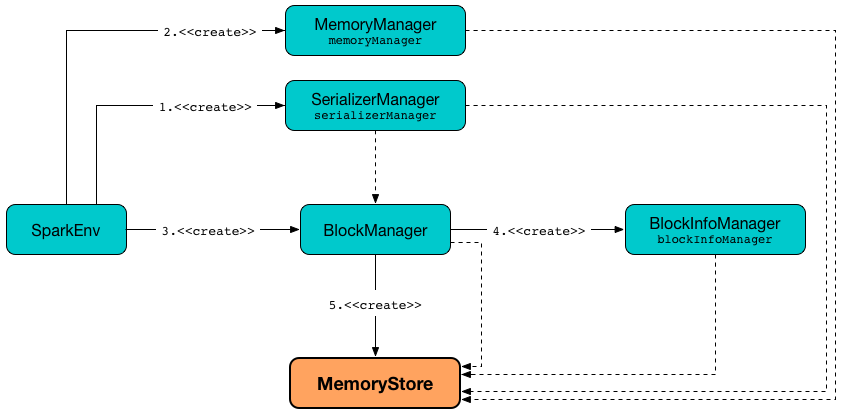
\includegraphics[scale=0.52]{imagens/criacao-memorystore.png}
    \end{center}
    \small{Fonte: \cite{laskowski2017mastering}}
    \label{fig:criacao-memorystore}
\end{figure}

A classe \textit{SerializerManager} é responsável por configurar o serializador utilizado pelo Spark, incluindo aquele utilizado nas operações de \textit{shuffle}. Esta classe é utilizada para a criação do \textit{BlockManager} e do \textit{MemoryStore}.

A classe \textit{BlockManager} oferece interfaces para realizar a adição e recuperação de blocos de dados localmente no \textit{Executor} e remotamente, isto é, em outros nodos do \textit{cluster} \cite{BlockManagerSpark}. A adição e recuperação desses blocos pode ser realizada em diferentes fontes de armazenamento, tais como memória principal e armazenamento estável.

O \textit{BlockManager} é responsável também, pela criação do \textit{BlockInfoManager} a qual tem como objeto rastrear os metadados dos blocos de dados de maneira individual, os quais são utilizados para informar a localização do bloco, isto é, memória ou disco. Ainda, é função do \textit{BlockInfoManager} fornercer os \textit{locks} de leitura e escrita desses blocos.

Na classe \textit{MemoryStore} encontram-se os métodos e variáveis para armazenamento e remoção de informações da memória \cite{MemoryStoreSpark}. Estas informações podem ser \textit{Arrays} de objetos Java desserializados ou \textit{Buffers} de \textit{bytes} serializados. Além disso, cabe a esta classe implementar a política de gerenciamento de memória utilizada pelo Spark: o algoritmo LRU.

O LRU é um algoritmo clássico para gerenciamento de memória em diversos sistemas. No Spark, a implementação deste algoritmo é realizada utilizando uma lista encadeada (\textit{LinkedHashMap}) provida nativamente pela distribuição Java. Através desta estrutura, o Spark mantém uma estrutura de lista encadeada contendo os dados de maneira ordenada por acesso. Cada vez que uma determinada posição dessa lista é acessada, esta posição é movida para o final da lista. Por consequência, as posições mais recentemente acessadas são encontradas ao final desta lista encadeada.

A estrutura de lista é iniciada com 32 posições e um fator de carregamento de 75\%. Isso significa que, ao atingir 75\% da capacidade de ocupação, novas posições começam a ser alocadas dinamicamente pela JVM. Uma particularidade dessa lista está relacionada à forma como a mesma deve ser manipulada em ambientes \textit{multithread}. Nesses ambientes, o acesso deve ser feito de maneira sincronizada entre as \textit{threads} em execução, pois a implementação não é realizada de maneira \textit{thread-safe}. Essa sincronização busca manter a ordenação, uma vez que há alteração nas posições armazenadas na lista quando ocorre acesso a mesma.

A sincronização entre as \textit{threads} em execução no Spark é realizada através de um \textit{lock} global do objeto. Deste modo, apenas uma \textit{thread} consegue realizar a escrita, leitura ou remoção de um bloco de dado a partir da estrutura, evitando condições de corrida (\textit{race condition}) entre as \textit{threads}. Entretanto, esta sincronização pode acarretar em uma sobrecarga para a aplicação, uma vez que durante essas operações apenas uma \textit{thread} consegue manipular a estrutura, bloqueando as demais.

Cada Spark \textit{Worker} executando no \textit{cluster} possui suas próprias estruturas para controlar as regiões de memória. Assim, cada nodo Spark gerencia sua memória de forma autônoma e sem dependências externas. Além disso, devido à distribuição dos dados do RDDs entre os nodos, o momento em que blocos de memória deverão ser removidos pode variar entre diferentes nodos. 

\section{Apache ZooKeeper} \label{sec:Zookeeper}
O Apache ZooKeeper é um \textit{framework} de código aberto cujo objetivo é prover soluções para problemas de coordenação em grandes conjuntos de nodos \cite{hunt2010Zookeeper}. Através deste, é possível coordenar grupos de nodos entre si e manter o compartilhamento de informações com técnicas de sincronização robustas.

O ZooKeeper realiza o processo de coordenação através de um \textit{namespace} hierárquico compartilhado organizado de maneira semelhante a um sistema de arquivos padrão. Entretanto, diferente dos sistemas de arquivos, os nodos responsáveis por armazenar os dados, denominados de \textit{znodes}, são estruturas similares a arquivos e diretórios projetados para serem armazenados em memória principal. Um \textit{namespace} do \textit{znode} pode conter dados associados e referências a outros \textit{znodes}.  A Figura \ref{fig:ZookeeperNamespace} exibe um nodo denominado de \textit{"/"}, o qual possui dois outros nodos associados, exemplificando a arquitetura utilizada no \textit{namespace}.

\begin{figure}[!ht]
    \caption{Estrutura de \textit{namespace} do Apache ZooKeeper}
    \begin{center}
        \includegraphics[scale=0.5]{imagens/Zookeeper-namespace.png}
    \end{center}
    \small{Fonte: \cite{haloi2015apache}}
    \label{fig:ZookeeperNamespace}
\end{figure}

Um \textit{znode} mantém uma estrutura do estado atual dos dados armazenados, a qual inclui o número da versão, o \textit{Action Control List} (ACL) e um \textit{Timestamp}. O número da versão representa a quantidade de vezes que os dados armazenados pelo \textit{znode} foram alterados.  O ACL é o mecanismo de autenticação, assegurando quais nodos do \textit{cluster} podem realizar operações de escrita e leitura. O \textit{Timestamp} descreve o tempo decorrido desde a criação do nodo até o momento da modificação dos dados armazenados. 

Uma importante característica do ZooKeeper é a capacidade de oferecer suporte a \textit{Watchers}, permitindo que clientes possam receber notificações ocorridas em um determinado \textit{znode}. A manutenção da comunicação entre o \textit{Master} e os clientes é realizada através de mensagens \textit{heartbeat}, as quais garantem que a conexão com os clientes entra-se ativa.

Uma mudança em um \textit{znode} consiste em uma modificação nos dados associados a este nodo ou uma alteração em um de seus nodos filhos \cite{junqueira2013Zookeeper}. Através dos \textit{znodes}, as aplicações podem oferecer suporte a serviços de sincronização, fila de mensagens, além de gerenciamento de configuração do \textit{cluster}.

Juntamente com seu sistema de \textit{znodes}, o ZooKeeper oferece uma API com suporte oficial para as linguagens Java e C, a fim de realizar a criação de aplicações cliente. Através destes clientes, pode-se conectar, manipular dados associados aos \textit{znodes}, coordenar operações e interagir com ZooKeeper.


\section{Trabalhos Relacionados} \label{sec:trab-relacionados}
O algoritmo utilizada para o gerenciamento do espaço disponível pode afetar diretamente o desempenho do \textit{framework} durante o processamento de aplicações. Nesse sentido, alternativas têm sido pesquisadas e desenvolvidas buscando aumentar a eficiência do Apache Spark.

O trabalho desenvolvido por \cite{wang2015new} apresenta uma abordagem para analisar o comportamento do Spark ao realizar acessos à memória visando melhorar a ordem da execução de ações nos RDDs. Para tanto, os autores utilizam um algoritmo guloso para encontrar a melhor sequência para executar as ações aplicadas aos RDD, uma vez que o processamento de uma ação independe das demais. Juntamente com este algoritmo, a abordagem tem como objetivo calcular um peso do RDD em uma \textit{task}. O cálculo deste peso considera 6 critérios: tamanho dos dados de entrada do RDD, custo de computação, frequência de reutilização, tamanho do conjunto de dados de saída da transformação aplicada, ciclo de vida do RDD (isto é, por quanto tempo este é manipulado) e custo de armazenar o RDD em disco. Em seguida, é apresentado um novo algoritmo denominado de ASRD (\textit{Action's Sequence and RDD Weight}), o qual combina a análise da execução aliada ao peso do RDD calculado. Os autores não especificam a versão do Spark utilizada, tampouco o ambiente usado para validação do método proposto. Entretanto, os autores do trabalho não apresentaram resultados em termos percentuais, limitando-se a afirmar que a metodologia proposta obteve um ganho na taxa de acerto de acesso à memória, quando comparado ao LRU.

Em \cite{duan2016selection} é  apresentado um algoritmo para a seleção de RDDs a serem armazenados em \textit{cache} baseado na frequência de utilização dos RDDs na aplicação. Dessa forma, remove-se a necessidade do desenvolvedor de decidir qual RDD deve ser mantido em \textit{cache} para ser reutilizado posteriormente. Quando a memória alcança o seu limite disponível, blocos são removidos de acordo com uma nova política proposta pelos autores: o algoritmo \textit{Weight Replacement}. Esse algoritmo consiste na atribuição de um peso, calculado a partir do custo de recomputação da partição, além da frequência de utilização e tamanho da partição. A proposta apresentada foi implementada no Spark 1.1.0 e validada utilizando 17 \textit{datasets} reais. De acordo com os autores, o algoritmo proposto obteve melhores resultados quando comparado ao LRU, reduzindo o tempo de execuçāo da aplicação \textit{PageRank}. Entretanto, não são apresentados percentuais deste ganho de desempenho. 

Em \cite{zhang2017intelligent}, os autores apresentam uma estratégia inteligente para \textit{checkpointing} e remoção de blocos da memória pelo Spark. Tal estratégia consiste na atribuição de uma prioridade \textit{P} para cada RDD, calculada a partir do tempo de recomputação, do tempo de \textit{checkpointing} e do grau de dependência entre os RDDs. Assim, quanto maior o valor de \textit{P}, maior deve ser a prioridade do RDD permanecer em memória. A validação desta proposta foi realizada utilizando o Spark 1.5 em 4 servidores, com a memória variando entre 5G, 10G e 20G. De acordo com os autores do trabalho, o resultado obtido demonstra um ganho médio de desempenho de 13,63\% quando comparado ao LRU.

O trabalho realizado por \cite{xu2016neutrino} apresenta um gerenciador de \textit{cache} distribuído denominado de \textit{Neutrino}. Esse gerenciador é responsável por tomar decisões relativas ao armazenamento dos RDDs com base em configurações do \textit{cluster} e na execução da aplicação. Para tanto, o \textit{Neutrino} analisa a ordem em que os RDDs serão utilizados e calcula o menor tempo de execução possível do \textit{Job}. Esse gerenciador foi implementado como uma extensão do Spark 1.5.0. De acordo com os autores, a solução proposta apresenta resultados promissores quanto a sua utilização. 

Em \cite{geng2017lcs} é demonstrada uma estratégia denominada \textit{Least Cost Strategy} (LCS) para a remoção de blocos de memória, a qual integra o custo de recuperação da partição em cache e a lógica de execução da aplicação. Este algoritmo combina o tempo necessário para criar, remover e recomputar cada partição dos RDDs juntamente com uma frequência de reutilização de cada partição. A implementação dessa estratégia foi realizada utilizando o Spark 1.5.2. Conforme os autores, o LCS consegue um desempenho em torno de 30\% melhor que o LRU.

Em \cite{yang2018intermediate}, os autores apresentam um algoritmo para determinar e armazenar adaptativamente os \textit{datasets} intermediários mais valiosos, isto é, aqueles que poderão ser reutilizados no futuro. Assim, este algoritmo automatiza a decisão de quais RDDs devem ser persistidos em memória, analisando o DAG gerado pelo Spark durante a execução do \textit{job}. O algoritmo foi implementado utilizando o Spark 2.2.1 e sua validação ocorreu utilizando a aplicação \textit{Ridge Regression}. Segundo os autores, o algoritmo proposto consegue reduzir em 12\% o trabalho necessário para realizar as recomputações dos RDDs removidos.

No trabalho desenvolvido por \cite{inagaki2018adaptive}, é apresentada uma metodologia de \textit{cache} adaptativa para o Spark, a qual modifica o comportamento dos métodos de armazenamento e remoção de dados da \textit{cache}, dependendo das características da aplicação. Em situações onde os dados da aplicação são frequentemente movidos da memória para o disco, esta abordagem de \textit{cache} adaptativo move estes dados diretamente para o armazenamento estável. Além disso, se estes dados armazenados no disco são requeridos pela aplicação, o mecanismo de \textit{cache} adaptativo carrega os dados necessários diretamente para a Memória de Execução do Spark. Estas ações de carga de \textit{cache} são realizadas analisando a execução da aplicação ao invés das dependências entre os RDDs. A implementação desta estratégia foi realizada utilizando a versão 2.0.1 do Spark. De acordo com os autores, este mecanismo de gerenciamento de \textit{cache} reduziu em 33\% o tempo de execução do \textit{benchmark} K-Means, quando comparado ao LRU utilizando o nível de armazenamento Memória e Disco nativo do Spark. 

É possível encontrar na literatura algoritmos e soluções que têm como objetivo melhorar a forma na qual o Spark realiza o processamento de aplicações onde há a reutilização de dados em computações futuras, uma vez que o algoritmo LRU pode acarretar em degradação no desempenho do \textit{framework} nesta classe de aplicações. Entretanto, quando analisamos tais soluções, duas características ficam evidentes: versão do Spark e metodologia utilizada. 

A primeira característica está relacionada à versão utilizada para implementação e validação, onde geralmente os trabalhos concentram-se em versões defasadas e com um modelo de memória diferente daquela utilizada por versões mais novas do Spark. A segunda característica encontrada em trabalhos disponíveis na literatura relaciona-se com as soluções propostas, onde comumente foca-se em algoritmos estáticos e reativos. Embora as soluções encontradas utilizem métricas colhidas a partir da aplicação, estas soluções tendem a executar apenas quando há necessidade de liberação de memória.

Diferentemente dos algoritmos e soluções encontradas na literatura, este trabalho tem como objetivo implementar um modelo para realizar o Gerenciamento Dinâmico da Memória utilizada pelo Spark, em versões 2.x do \textit{framework}. Esta solução tem como foco as aplicações onde há reutilização de dados em computações futuras. Para tanto, o modelo proposto é composto por dois componentes: um algoritmo de gerenciamento de memória e um agente de monitoramento.

O algoritmo de gerenciamento de memória visa extrair a frequência de reutilização dos RDDs da aplicação e combiná-la com o algoritmo LRU. Já o agente de monitoramento tem como objetivo obter o \textit{status} e informações da aplicação em execução e decidir se deve ocorrer a remoção dos dados em \textit{cache}. Através deste modelo, busca-se corrigir as deficiências encontradas no algoritmo LRU no processamento de aplicações onde há reutilização de dados.